% !TEX root = ../thesis.tex
\graphicspath{{\aiaadir /figures_RANS_naca0012/}}% Set graphics path location

\subsection{NACA 0012 airfoil at 0$\degr$ angle of attack, Re = 6 million, Ma = 0.15}
In this section, the NACA 0012 airfoil is used to study the accuracy of the \gls{sa} turbulence model coupled with \gls{fr}. The NACA 0012 is commonly used as a validation case for all turbulence models and a large database of results are available at the NASA Turbulence Modeling Resource website. A $6,539$ element quad/triangle mixed mesh is used with a NACA 0012 airfoil of chord length $1.0$ and a far field boundary $20$ chord lengths away. The results are compared with CFL3D and experimental results from Gregory \& O'Reilly~\cite{gregory1973low}.

\begin{figure}

    \subfloat[Zoomed view of the mixed element mesh near the NACA 0012 airfoil.]{\includegraphics[width = 0.5\textwidth]{NACA0012_Re6mil_mesh.eps}}
    \subfloat[X-momentum contours near the NACA 0012 airfoil]{\includegraphics[width = 0.5\textwidth]{NACA0012_Re6mil_alp0_momx.eps}}

  \caption{Turbulent flow past a NACA 0012 airfoil at \gls{re} = 6 million, \gls{ma} = 0.15, $\alpha = 0^{\circ}$ using \gls{fr} to recover 4th order accurate \gls{dg} method and the \gls{sa} turbulence model.}
  \label{RANS_naca0012}
\end{figure}

\begin{figure}
\centering
  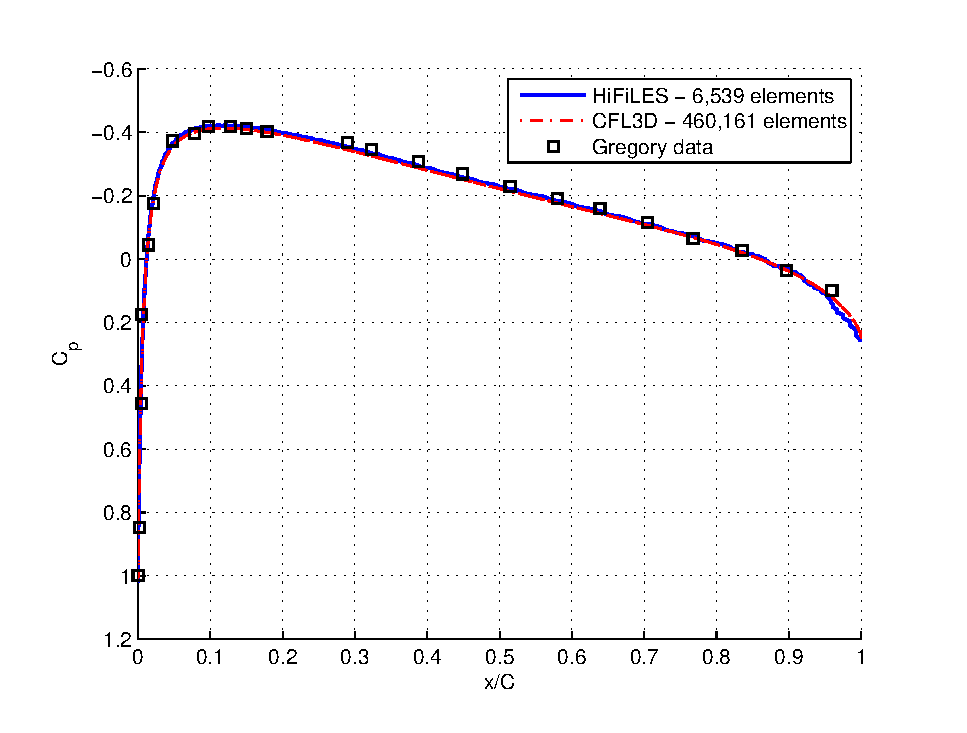
\includegraphics[width=0.48\textwidth]{cp.eps}
  \caption{Pressure coefficient on the NACA 0012 airfoil at \gls{re} = 6 million, \gls{ma} = 0.15, $\alpha = 0^{\circ}$ using \gls{fr} to recover 4th order accurate \gls{dg} method and the \gls{sa} turbulence model.}
  \label{RANS_naca0012_cp}
\end{figure}

